\section{The Problem and Its Importance}\label{sec:problem}

\subsection{A person, not an abstraction}

Consider a real profile from the Gangshan cluster: a second-generation owner in
his sixties, thirty employees, precision screws for European automotive
distributors, administration handled by his daughter-in-law on a spreadsheet.
Nationally, 51.79\% of Taiwan's SMEs are exactly this --- sole proprietorships
or family firms, most over eight years old\cite{moea}. His factory is one of
$\sim$1,800 in a district that ships roughly 1.2 million tonnes of fasteners a
year and holds 10--13\% of world production --- a top-three global
exporter\cite{ktimes,goebel}, a quarter of it bound for Europe\cite{cw}.

In January 2026 his largest buyer's procurement system began scoring him on a
number he has never produced: the verified carbon content of his screws. Sector
surveys show how unprepared his cohort is: \textbf{60\%} of fast-growing SMEs
have completed no carbon inventory, \textbf{80\%} have no reduction targets,
and half name talent shortage as the binding constraint\cite{cw}.

\subsection{The mechanism that turns ignorance into lost orders}

The EU's Carbon Border Adjustment Mechanism entered its paying phase on
1~January~2026: importers of steel goods (including screws and bolts, CN~7318)
must surrender certificates priced at the official EU rate --- EUR~75.36 in
Q1, EUR~75.28 in Q2 2026\cite{taxud,ecprice,carbonchain}. With verified data,
a tonne of fasteners ($\sim$2~tCO$_2$e embedded\cite{specialinsert}) costs the
buyer about \textbf{EUR~150}. Without it, punitive default values apply ---
3--5$\times$ higher by industry estimate, marked up a further 10\% this year
and 30\% by 2028\cite{omm,specialinsert} (Figure~\ref{fig:cbamcost2}). Analysts
put worst-case exposure at \textbf{30--50\% of product value} on commodity
lines\cite{specialinsert}. The 50-tonne exemption does not save the small: it
is counted per \emph{EU importer}, cumulatively across all suppliers ---
MOENV's Climate Change Administration has warned publicly that even
minimal-volume Taiwanese SMEs will be swept in\cite{tpt-cbam}.

\begin{figure}[htbp]
\centering
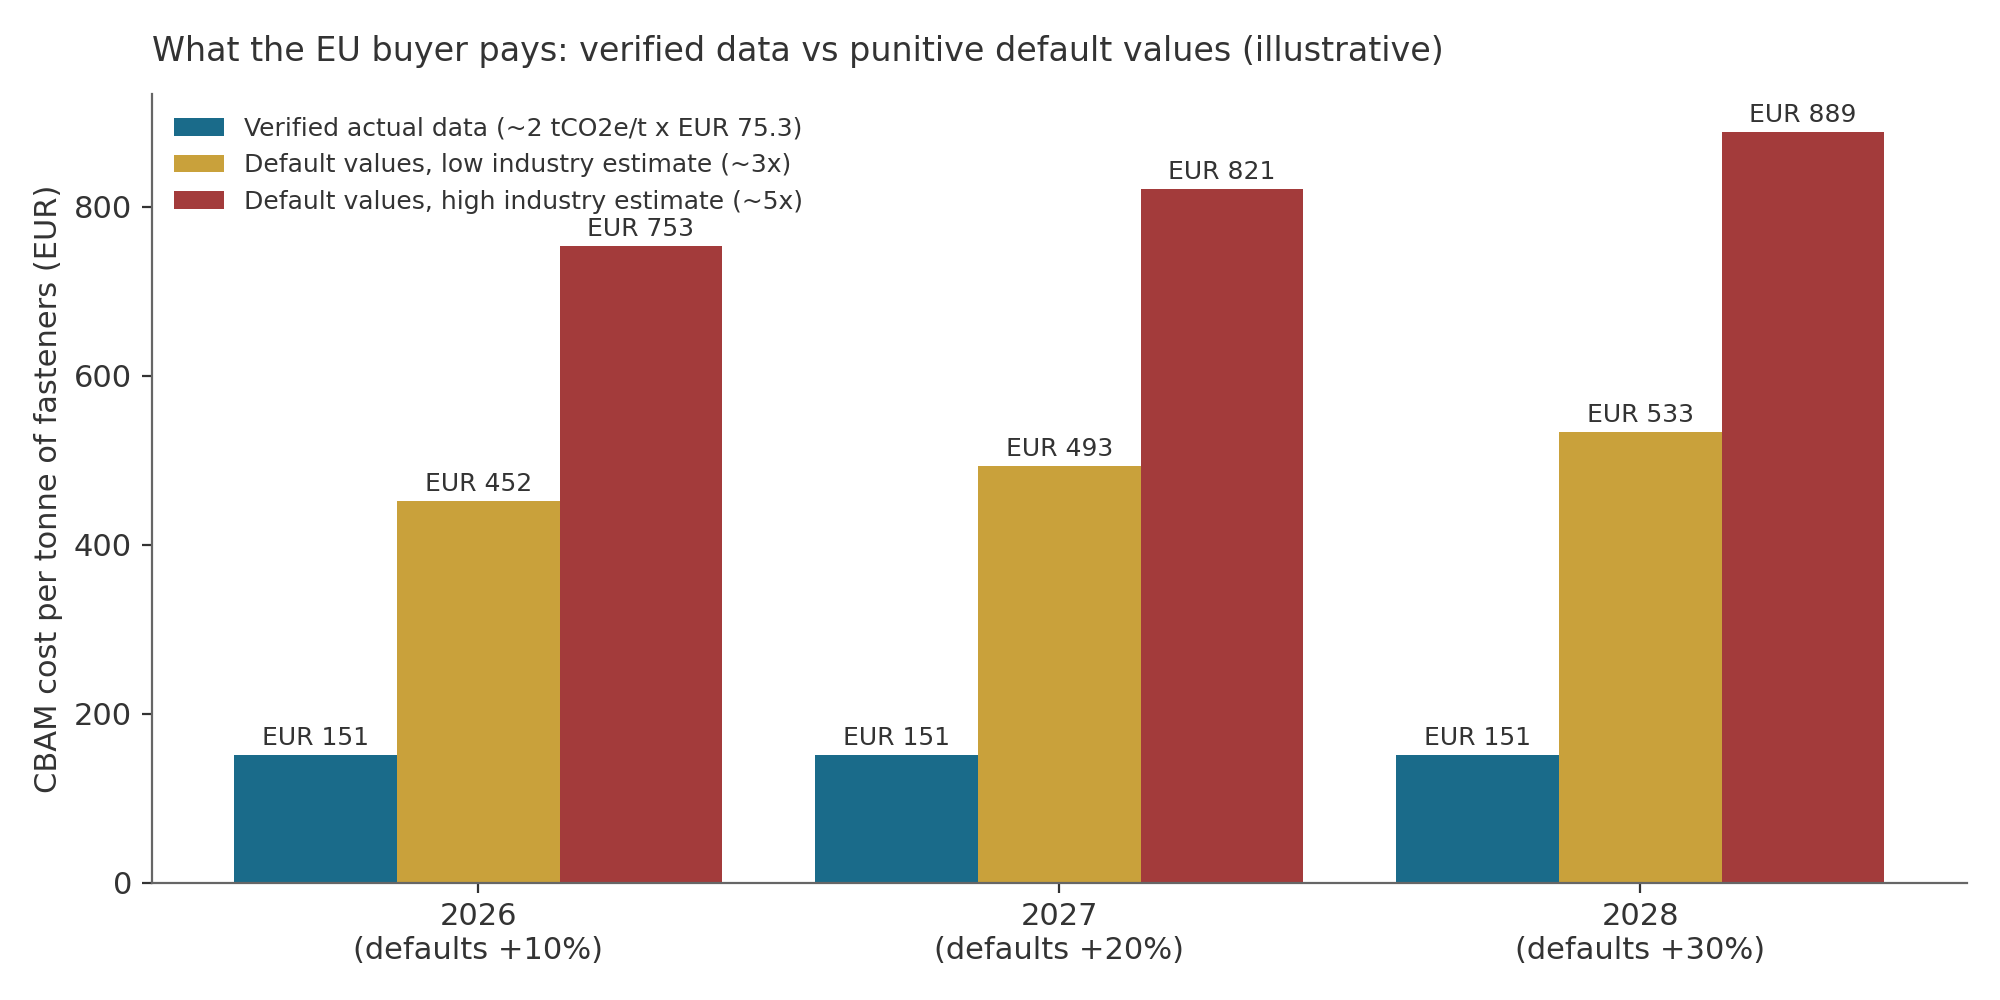
\includegraphics[width=0.93\textwidth]{chart3_cbam.png}
\caption[The price of missing data: verified vs.\ default CBAM costs]{What the
EU buyer pays per tonne of Taiwanese fasteners: verified actual data versus
punitive defaults, at the official certificate price\cite{ecprice}, with the
regulation's automatic markup escalation\cite{omm}. The gap is the survival
margin of a family factory.}
\label{fig:cbamcost2}
\end{figure}

MOENV counts \textbf{$\sim$2,600 Taiwanese SMEs} producing the affected goods
--- 3.74 million tonnes shipped to the EU in the last reporting
period\cite{tpt-cbam} (Figure~\ref{fig:funnel2}).

\begin{figure}[htbp]
\centering
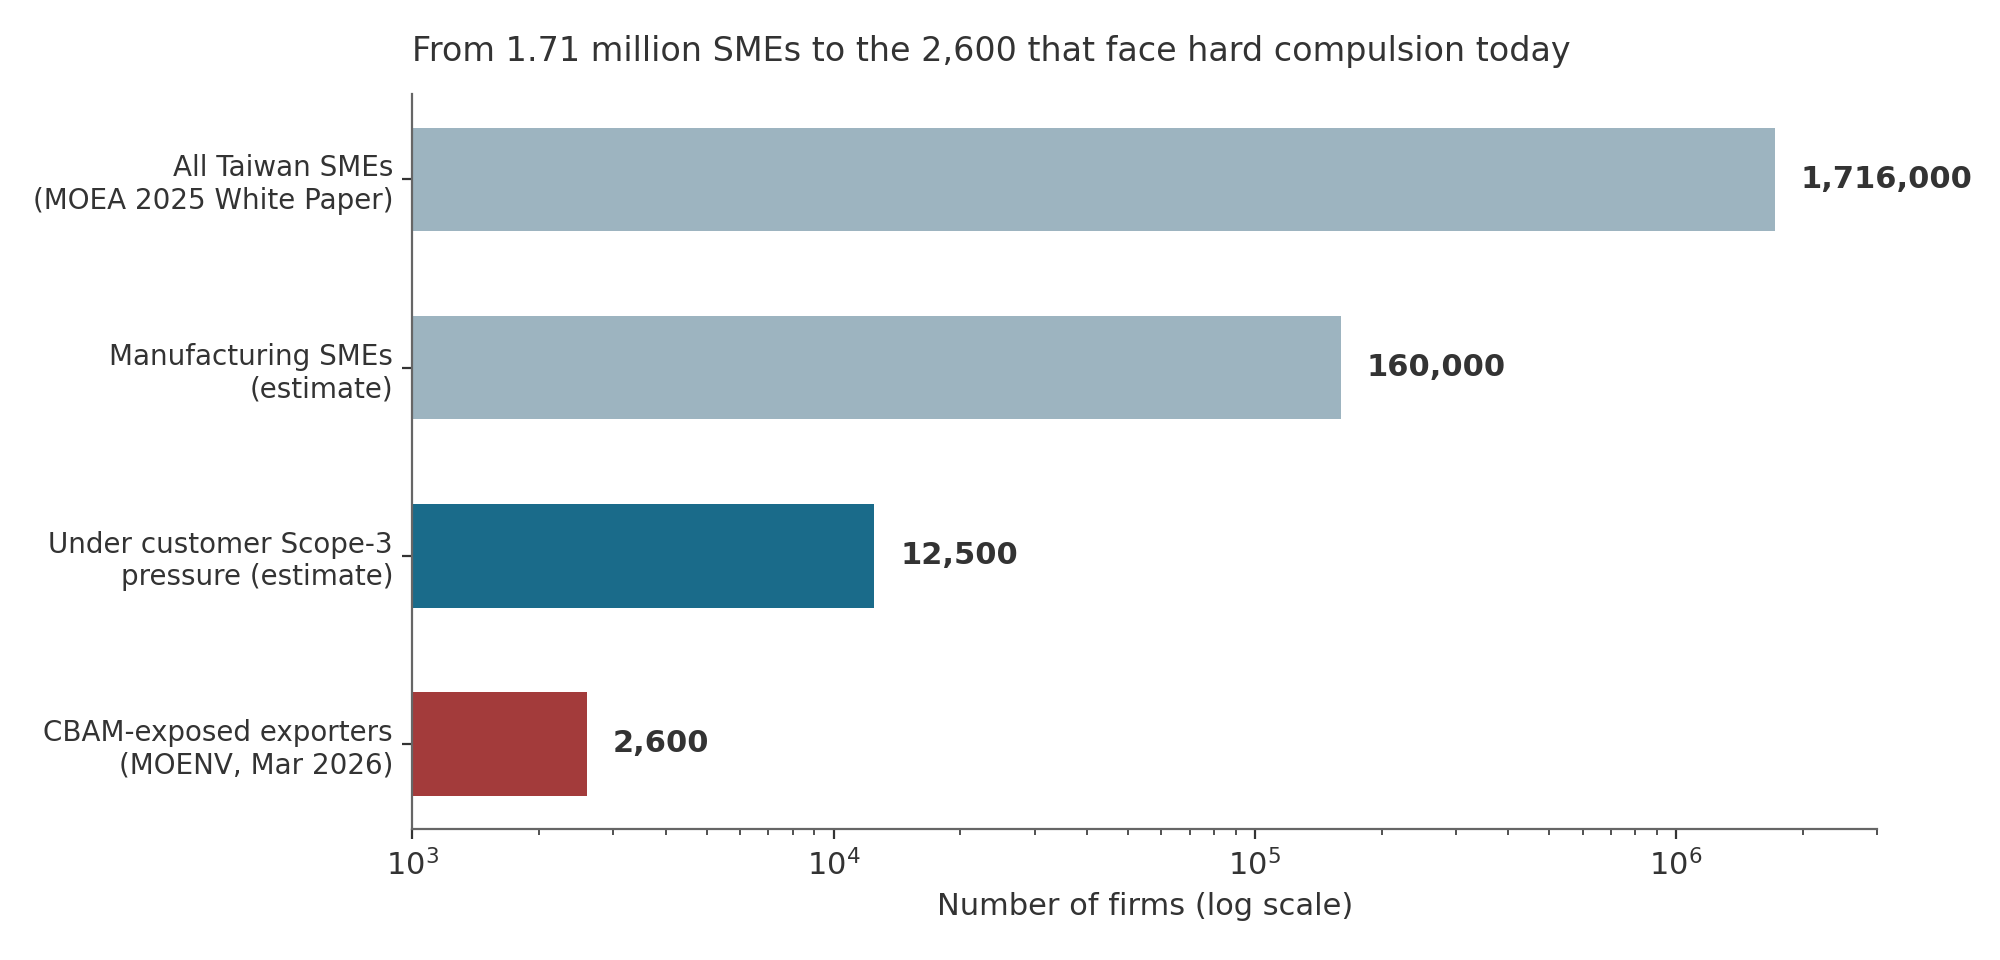
\includegraphics[width=0.93\textwidth]{chart1_funnel.png}
\caption[A precisely targeted population, not an inflated one]{This proposal
targets a precisely named population, not an inflated one: of Taiwan's 1.716
million SMEs\cite{moea}, the ones facing hard compulsion today are the
$\sim$2,600 CBAM-exposed exporters identified by MOENV\cite{tpt-cbam}. Middle
bars are our estimates of the wider customer-pressured band.}
\label{fig:funnel2}
\end{figure} Behind the firms stand the jobs, suppliers, and the
economic identity of an entire southern district. And the wall is still
rising: the European Parliament votes in September 2026 on extending the
mechanism to $\sim$180 further steel and aluminium product categories from
2028\cite{akin}, while at home the carbon-fee threshold will fall and an
emissions-trading pilot approaches\cite{ecobiz}. \textbf{This problem is not a
wave but a rising floor} --- and the population it lands on first has already
been named by the government itself.

\section{Digital Inclusion, Exactly as the Handbook Defines It}\label{sec:inclusion}

The Handbook's first objective asks entries to enable ``\emph{people of
different ages, regions, and needs} to access technology and participate in
digital services on equal footing, thereby narrowing the digital
divide''\cite{handbook}. CarbonPass answers each axis literally:

\begin{description}[leftmargin=1.2em,style=nextline]
\item[Ages.] The population being excluded is demonstrably older and
analog-native: family firms run by senior owner-operators, back offices
without a single data professional\cite{moea,cw}. They are being asked to
operate EU-grade data infrastructure overnight. CarbonPass meets them where
they are: a voice-friendly conversation in LINE, in Mandarin and Taiwanese ---
``{\cjk 拍一張電費單}'' (\emph{snap a photo of the power bill}) is the entire
onboarding.
\item[Regions.] The excluded community is geographically concrete: the
Gangshan--Luzhu district of Kaohsiung, whose industrial identity --- the
Kingdom of Screws --- is what the data wall threatens. Serving it is regional
inclusion in the most literal sense.
\item[Needs.] Carbon-verified market access has become a de facto
\emph{digital service}: participate or be de-listed. Today only corporations
can afford to participate. CarbonPass extends that participation to a
12-person factory at near-zero marginal cost --- equal footing, in the
Handbook's own words.
\end{description}

The second objective --- ``building smarter services \ldots{} across
education, care services, governance, disaster prevention, \emph{and
beyond}''\cite{handbook} --- is answered by what the system does with public
infrastructure: it turns Taiwan's open data (emission coefficients, grid
telemetry, tariffs) into a service layer that the government's own CBAM help
platform currently lacks\cite{tpt-cbam}. \textbf{Where earlier editions of
this competition bridged the divide of broadband and the divide of
disability, 2026's sharpest divide is the data divide --- and it can be
bridged the same way: by putting AI on the excluded side of the wall.}
